\section{Vzorkování z latentního prostoru}

\begin{figure}[H]
    \centering
    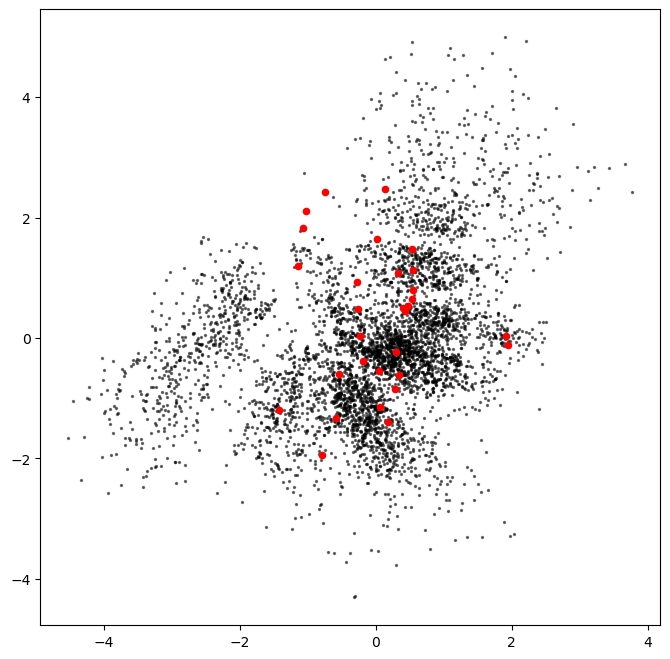
\includegraphics[width=0.8\textwidth]{figures/vae_sampling_latent_space.png}
    \caption{Vzorkování z latentního prostoru naučeného modelu. Červené body značí bod z latentního prostoru, který byl použit jako vstup pro dekodér modul.}
\end{figure}

\autoref{fig:vae_sampling_results} vzorky vygenerované naučeným modelem. Lze si povšimnout, že většina vygenerovaných číslic \textbf{není deformovaná}.
To je důsledek \textbf{lokální spojistosti latentního prostoru} (v kontrastu s prostým autoenkodérem, jehož latentní prostor je nespojitý).

\begin{figure}[H]
    \centering
    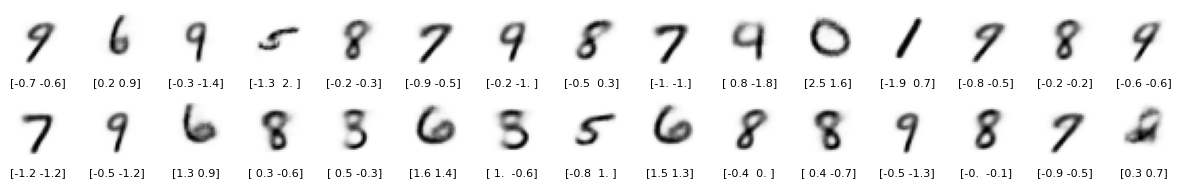
\includegraphics[width=\textwidth]{figures/vae_model_sampling_latent_space_results.png}
    \caption{Vzorky vygenerované naučeným modelem variačního autoenkodéru.}
    \label{fig:vae_sampling_results}
\end{figure}